\documentclass{article}
\usepackage[utf8]{inputenc}
\usepackage{amsmath}
\usepackage{amssymb}
\usepackage{parskip}
\usepackage{dsfont}
\usepackage{fullpage}
\usepackage{pgfplots}

\title{Euler's Formula}
\author{Paolo Bettelini}
\date{}

\begin{document}

\maketitle
\tableofcontents
\pagebreak

\section{Definition}

Euler's formula states that for every \(x\in\mathbb{R}\)
\begin{align*}
    e^{ix}=cos\,x+i\,sin\,x
\end{align*}

We can represent the formula on the complex plane

\begin{center}
    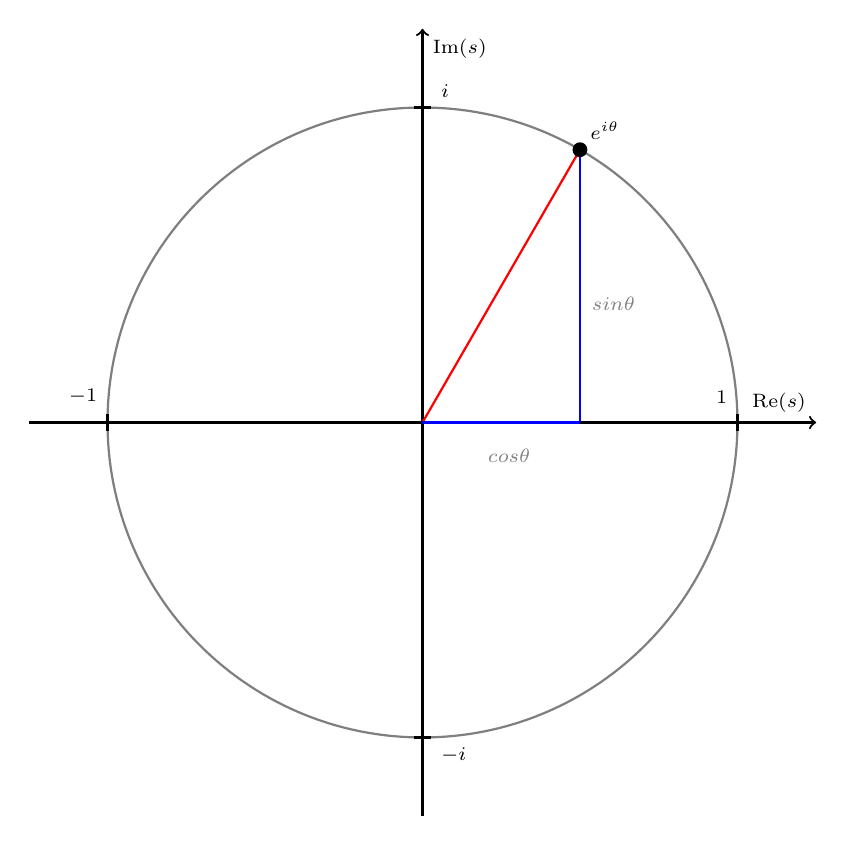
\begin{tikzpicture}
        \begin{scope}[thick, font=\scriptsize, scale=4]
            \draw [->] (-1.25,0) -- (1.25,0) node [above left]  {Re(\(s\))};
            \draw [->] (0,-1.25) -- (0,1.25) node [below right] {Im(\(s\))};
        
            \draw (1,-0.75pt) -- (1,0.75pt)   node [above left] {$1$};
            \draw (-1,-0.75pt) -- (-1,0.75pt) node [above left] {$-1$};
            \draw (-0.75pt,1) -- (0.75pt,1)   node [above right] {$i$};
            \draw (-0.75pt,-1) -- (0.75pt,-1) node [below right] {$-i$};

            \path [draw=black,fill=none,semitransparent] (0, 0) circle (1);
            \draw [thick, color=red] (0,0) -- (0.5,0.866);
            \draw [thick, color=blue] (0.5,0) -- (0.5,0.866);
            \draw [thick, color=blue] (0,0) -- (0.5,0);
            
            \draw [color=black, fill=black] (0.5,0.866) circle(0.02) node [above right] {\(e^{i\theta}\)};
            
            \node [below right,gray] at (0.175, -0.05) {\(cos\theta\)};
            \node [below right,gray] at (0.505, 0.43) {\(sin\theta\)};
        \end{scope}
    \end{tikzpicture}
\end{center}

We can notice that \(\left|e^{ix}\right|=1\) since \(e^{i\theta}=cos^2\theta +sin^2\theta =1\)

\section{Proof}

To understand this identity we must first look at the Taylor series of some functions.

\subsection{Sine function}
\subsection{Cosine function}
\subsection{Exponential function}

\pagebreak

\subsection{Conclusion}

Given the Taylor series for the exponential function
\begin{align*}
    e^x=\sum_{n=0}^{\infty}\frac{x^n}{n!}
\end{align*}
we plug in \(ix\) instead of \(x\):
\begin{align*}
    e^{ix}=\sum_{n=0}^{\infty}\frac{(xi)^n}{n!}
\end{align*}
The imaginary number \(i\) has some amazing property when it comes to exponentiation.
\begin{align*}
    \begin{cases}
        i^0=+1\\
        i^1=+i\\
        i^2=-1\\
        i^3=-i\\
    \end{cases}
    \quad
    \begin{cases}
        i^4=+1\\
        i^5=+i\\
        i^6=-1\\
        i^7=-i\\
    \end{cases}
    \quad
    \cdots
\end{align*}
We can use these properties to simplify the \(e^{ix}\) Taylor series
\begin{align*}
    e^{ix}
    &   =1
        +ix
        +\frac{(ix)^2}{2!}
        +\frac{(ix)^3}{3!}
        +\frac{(ix)^4}{4!}
        +\frac{(ix)^5}{5!}
        +\frac{(ix)^6}{6!}
        +\frac{(ix)^7}{7!}
        +\cdots
    \\
    \\
    &   =1
        +ix
        -\frac{x^2}{2!}
        -\frac{ix^3}{3!}
        +\frac{x^4}{4!}
        +\frac{ix^5}{5!}
        -\frac{x^6}{6!}
        -\frac{ix^7}{7!}
        +\cdots
    \\
    \\
    &=
    \left(
        1
        -\frac{x^2}{2!}
        +\frac{x^4}{4!}
        -\frac{x^6}{6!}
        +\cdots
    \right)
    +i
    \left(
        x
        -\frac{x^3}{3!}
        +\frac{x^5}{5!}
        -\frac{x^7}{7!}
        +\cdots
    \right)
\end{align*}
We notice that the two terms correspond to the sine and cosine Taylor series
\begin{align*}
    e^{ix}=cos\,x+i\,sin\,x
\end{align*}

\end{document}